\documentclass[reqno,12pt,oneside]{report} % right-side equation numbering, 12 point font, print one-sided
%\documentclass[reqno,12pt,twoside,openright]{report} % right-side equation numbering, 12 point font, print two-sided, Chapters start on odd pages. Rackham only accepts one-sided, so this is for personal printings.

\usepackage{rac}         % Use Rackham thesis style file
%\usepackage{aas_macros}  % To allow the reading of ADS journal references in the bibliography
\usepackage[intlimits]{amsmath} % Puts the limits of integrals on top and bottom
\usepackage{amsxtra}     % Use various AMS packages

\usepackage{amsthm}
\usepackage{amssymb}
\usepackage{graphicx}    % Add some packages for figures. Read epslatex.pdf on ctan.tug.org

\usepackage{rotating}
\usepackage{color}
\usepackage{xspace}
\usepackage{mdframed}
\usepackage{epsfig}
\usepackage{subfigure}   % To make subfigures. Read subfigure.pdf on ctan.tug.org
\usepackage{multirow}

\usepackage{verbatim}
\usepackage[numbers]{natbib}      % Allows you to use BibTeX
\usepackage{acronym} % For the List of Abbreviations. Read acronym.pdf on ctan.tug.org
\usepackage{booktabs}% http://ctan.org/pkg/booktabs
\newcommand{\tabitem}{~~\llap{\textbullet}~~}
\usepackage{indentfirst}
\usepackage{enumitem}
\usepackage{setspace}
\usepackage[T1]{fontenc}
\usepackage[utf8]{inputenc}
%\usepackage[options ]{algorithm2e}
\usepackage{algpseudocode}
\usepackage{ifthen}
%\usepackage{mathptmx} 
%\usepackage[acronym]{glossaries}
%\usepackage{nomencl}
%\usepackage[noend]{algpseudocode}
%\usepackage[linesnumbered,ruled,vlined]{algorithm2e}

\usepackage[intoc]{nomencl}
\usepackage{tikz}
\usetikzlibrary{shapes.geometric, arrows}

\usepackage{url}
%\usepackage{breakurl}
%\usepackage[breaklinks]{hyperref}
\usepackage[colorlinks=true, allcolors=black]{hyperref}
 
\usepackage{algorithm,algpseudocode}
\usepackage[font=small,labelfont=bf]{caption}



%\usepackage[latin1]{inputenc}
%\usetikzlibrary{shapes,arrows}
\tikzstyle{startstop} = [rectangle, rounded corners, minimum width=3cm, minimum height=1cm,text centered, draw=black, fill=red!30]
\tikzstyle{io} = [trapezium, trapezium left angle=70, trapezium right angle=110, minimum width=3cm, minimum height=1cm, text centered, draw=black, fill=blue!30]
\tikzstyle{process} = [rectangle, minimum width=3cm, minimum height=1cm, text centered, draw=black, fill=orange!30]
\tikzstyle{decision} = [diamond, minimum width=3cm, minimum height=1cm, text centered, draw=black, fill=green!30]
\tikzstyle{arrow} = [thick,->,>=stealth]

%%%<


\usepackage[nottoc,notlof,notlot]{tocbibind}
\renewcommand\bibname{References}

\makenomenclature
%\makenomenclature
  % Allows you to specify the line spacing
%\doublespacing
\onehalfspacing %for 1.5 spacing, %\doublespacing for 2.0 spacing.
\newcommand{\sun}{\ensuremath{\odot}} % sun symbol is \sun
%%%%%%%%%%%%%%%%%%%%%%%%%%%%%%%%%%%%%%%%%%%%%%%%%%%%%%%%%%%%%%%%%%%%%%%%%%%%%%%

% Various theorem environments. All of the following have the same numbering
% system as theorem.

\theoremstyle{plain}
\newtheorem{theorem}{Theorem}
\newtheorem{prop}[theorem]{Proposition}
\newtheorem{corollary}[theorem]{Corollary}
\newtheorem{lemma}[theorem]{Lemma}
\newtheorem{question}[theorem]{Question}
\newtheorem{conjecture}[theorem]{Conjecture}
\newtheorem{assumption}[theorem]{Assumption}

\theoremstyle{definition}
\newtheorem{definition}[theorem]{Definition}
\newtheorem{notation}[theorem]{Notation}
\newtheorem{condition}[theorem]{Condition}
\newtheorem{example}[theorem]{Example}
\newtheorem{introduction}[theorem]{Introduction}

\theoremstyle{remark}
\newtheorem{remark}[theorem]{Remark}
%%%%%%%%%%%%%%%%%%%%%%%%%%%%%%%%%%%%%%%%%%%%%%%%%%%%%%%%%%%%%%%%%%%%%%%%%%%%%%%

\numberwithin{theorem}{chapter}     % Numbers theorems "x.y" where x
                                    % is the section number, y is the
                                    % theorem number

%\renewcommand{\thetheorem}{\arabic{chapter}.\arabic{theorem}}

%\makeatletter                      % This sequence of commands will
%\let\c@equation\c@theorem          % incorporate equation numbering
%\makeatother                       % into the theorem numbering scheme

%\renewcommand{\theenumi}{(\roman{enumi})}

%%%%%%%%%%%%%%%%%%%%%%%%%%%%%%%%%%%%%%%%%%%%%%%%%%%%%%%%%%%%%%%%%%%%%%%%%%%%%%

% If printing two-sided, this makes sure that any blank page at the
% end of a chapter will not have a page number.
\makeatletter
\def\cleardoublepage{\clearpage\if@twoside \ifodd\c@page\else
\hbox{}
\thispagestyle{empty}
\newpage
\if@twocolumn\hbox{}\newpage\fi\fi\fi}
\makeatother

%%%%%%%%%%%%%%%%%%%%%%%%%%%%%%%%%%%%%%%%%%%%%%%%%%%%%%%%%%%%%%%%%%%%%%%%%%%%%%

%This command creates a box marked ``To Do'' around text.
%To use type \todo{  insert text here  }.

\newcommand{\todo}[1]{\vspace{5 mm}\par \noindent
\marginpar{\textsc{To Do}}
\framebox{\begin{minipage}[c]{0.95 \textwidth}
\tt\begin{center} #1 \end{center}\end{minipage}}\vspace{5 mm}\par}



\begin{document}
%\bibliographystyle{ieeetr}
%\bibliographystyle{plain}    % Set the bibliography style. agu04, plain, alpha, etc.
% Title page as required by Rackham dissertation guidelines
\titlepage{\textbf{Predicting Dark Matter Presence Using Supervised Machine Learning}
}{232107}{Professional Masters in Information Technology}
{Information Technology}{September 2025}
{  Professor Dr. Risala Tasin Khan }

% Begin the front matter as required by Rackham dissertation guidelines
\initializefrontsections

% Optional Frontispiece
%\frontispiece{\includegraphics[width=6in]{Intro/Happy} Find a cool picture to go here.}

% Optional, but recommended, Copyright page
%\copyrightpage{Your Name}

% Page numbering. If you don't include a frontispiece or copyright page, you'll need to change this for two-sided printing.
\makeatletter
\if@twoside \setcounter{page}{4} \else \setcounter{page}{1} \fi
\makeatother

% Optional Dedication page
%\dedicationpage{To Our Beloved Parents}


%Optional declaration page
\startdeclarationpage
I hereby declare that this thesis is based on the results found by ourselves. Materials
of work found by other researcher are mentioned by reference. This thesis, neither in
whole nor in part, has been previously submitted for any degree.

\bigskip
\bigskip
\bigskip


\begin{tabular}{p{5cm}p{5cm}p{5cm}}
\centering
  % after \\: \hline or \cline{col1-col2} \cline{col3-col4} ...
     &  &   \\
     &  &   \\
     &  &   \\
  \rule{3.5cm}{1pt} & \rule{3.5cm}{1pt} & \rule{3.5cm}{1pt}\\
  S. M. JAHANGIR \\
  Roll: 232107\\

\end{tabular}

\label{declaration}


%Optional Certificate page
\startcertificatepage
The project titled “Predicting Dark Matter Presence in Galaxies Using Supervised Machine Learning” submitted by Student - S. M. JAHANGIR , ID: 232107, Session: Summer 23, has been accepted as satisfactory in partial fulfillment of the requirement for the degree of Professional Masters in Information Technology on the 11th of October 2025 

%\bigskip

\bigskip
\bigskip


\noindent \begin{tabular}{l}

  % after \\: \hline or \cline{col1-col2} \cline{col3-col4} ...
  \rule{4cm}{1pt} \\
  Professor Dr. Risala Tasin Khan \\ % replace it
  Supervisor\\

\end{tabular}


%Accepted and approved in partial fulfilment of the requirement for the degree Professional Master in Information Technology.


\begin{center}
   \textbf{BOARD OF EXAMINERS}
\end{center}
\noindent \begin{tabular}{lp{1cm}r}
\centering
  % after \\: \hline or \cline{col1-col2} \cline{col3-col4} ...
  \rule{4cm}{1pt}&\\
     Professor  Dr. M. Shamim Kaiser  \\
     Professor, IIT, JU  & & PMIT Coordination Committee  \\
     & &  \\
     \rule{4cm}{1pt}&\\
    Professor Dr. Risala Tasin Khan   & &Member, PMIT Coordination Committee   \\
     Professor, IIT, JU  & &\& Director, IIT\\
    & &  \\
     \rule{4cm}{1pt}&\\
    
 Professor Dr. Jesmin Akhter & &Member  \\
      Associate Professor, IIT, JU  & &PMIT Coordination Committee  \\
     &  \\
     \rule{4cm}{1pt}&\\
       Professor K M Akkas Ali  & &Member,
     \\
      Associate Professor, IIT, JU  & &PMIT Coordination Committee  \\
      &  \\
     \rule{4cm}{1pt}&\\
     Dr. Rashed Mazumder
  & &Member  \\
      Associate Professor, IIT, JU  & &PMIT Coordination Committee  \\
     
  %\rule{4cm}{1pt} & \rule{4cm}{1pt} & \rule{4cm}{1pt}\\
   

\end{tabular}


%\noindent \begin{tabular}{p{5cm}p{4cm}p{5cm}}
%\centering
  % after \\: \hline or \cline{col1-col2} %\cline{col3-col4} ...
   %  &  &   \\
    % &  &   \\
     %&  &   \\
  %\rule{4cm}{1pt} &  & \rule{3.5cm}{1pt}\\
  %Jesmin Akhter &   &K M Akkas Ali\\
  %Chairman &   &Member\\
   %  &  &   \\
    % &  &   \\
  %\rule{3.5cm}{1pt}& & \rule{3.5cm}{1pt}\\
   %Shamim Al Mamun&   &Prof. Dr. M. A. Mottalib \\
  %Member &   &Member (External) \\
%\end{tabular}


\label{Certificate}



% Optional Acknowledgements page
\startacknowledgementspage
I would like to extend my heartfelt gratitude to everyone who played a role in the successful completion of this thesis. I am especially thankful to  Dr. Risala Tasin Khan, a distinguished Professor at the Institute of Information Technology (IIT), Jahangirnagar University, for her invaluable guidance, thoughtful suggestions, and constant encouragement throughout this journey. Her generous provision of a rich collection of books, journals, and research materials greatly enhanced the quality of my work.

I am also deeply grateful to Dr. Risala Tasin Khan, Director of IIT, for her insightful advice and unwavering support. My sincere thanks go to all the esteemed faculty members of IIT for their helpful direction and encouragement. I also acknowledge and appreciate the contributions of those who, directly or indirectly, supported the successful completion of this research.

Finally, I would like to thank the administrative and support staff of IIT, Jahangirnagar University, as well as my friends, for their continuous encouragement and involvement throughout this academic journey.


\label{Acknowledgements}

%Optional Abstract page
\startabstractpage

Dark matter, accounting for a large part of the mass in the universe, yet elusive of detection in conventional observations because it does not interact with electromagnetic radiation. Prediction of the properties and dynamics of dark matter is hence a burning issue in astrophysics. In the following, we investigate the use of machine-learning (ML) approaches to predict dark matter properties from cosmological data and theory. Using many different supervised and unsupervised learning algorithms, such as decision trees, support vector machines or deep neural networks, we study a variety of input features including galaxy rotation curves, weak lensing data and cosmic microwave background measurements. Our results show that machine learning models can be used to infer patterns in large datasets which are the signature of dark matter distribution and characteristics, helping to shed light onto its elusive nature. Moreover, our predictive models give encouragingly accurate predictions for the dark matter density profiles and possible interactions with visible matter. This study highlights the power of ML in advancing the fundamental understanding of dark matter, serving as a harbinger for further research and experimental verification.


\vspace{8pt}
\textbf{Keywords:} Dark matter, machine learning, cosmological data, galaxy rotation curves, gravitational lensing, cosmic microwave background, prediction models, supervised learning, unsupervised learning, neural networks, astrophysics, density profiles, dark matter interactions, predictive modeling. 

 


\label{Abstract}




% List of Abbreviation

\listofabbreviations % Optional. Abbreviations should be stored in a file named abbr.tex
% Optional in-dissertation Abstract Page
%\startabstractpage
%{The Title of Your Dissertation}{Your Name}{Chair: Albert Einstein}
%
Dark matter, accounting for a large part of the mass in the universe, yet elusive of detection in conventional observations because it does not interact with electromagnetic radiation. Prediction of the properties and dynamics of dark matter is hence a burning issue in astrophysics. In the following, we investigate the use of machine-learning (ML) approaches to predict dark matter properties from cosmological data and theory. Using many different supervised and unsupervised learning algorithms, such as decision trees, support vector machines or deep neural networks, we study a variety of input features including galaxy rotation curves, weak lensing data and cosmic microwave background measurements. Our results show that machine learning models can be used to infer patterns in large datasets which are the signature of dark matter distribution and characteristics, helping to shed light onto its elusive nature. Moreover, our predictive models give encouragingly accurate predictions for the dark matter density profiles and possible interactions with visible matter. This study highlights the power of ML in advancing the fundamental understanding of dark matter, serving as a harbinger for further research and experimental verification.


\vspace{8pt}
\textbf{Keywords:} Dark matter, machine learning, cosmological data, galaxy rotation curves, gravitational lensing, cosmic microwave background, prediction models, supervised learning, unsupervised learning, neural networks, astrophysics, density profiles, dark matter interactions, predictive modeling. 

 


%\label{Abstract}

\section*{
\begin{center}
  LIST OF ABBREVIATIONS
\end{center}
}

\begin{tabular}{p{2.5cm}p{10cm}}
%\textbf{\symbab}  & \symbac\\

\textbf{SMV }  & Support Vector machine  \\
\textbf{KNN}  & K-Nearest Neighbors \\ 
% double back slash refers to newline
\textbf{LR}  & Logistic Regression\\
\textbf{ROC}  & The Receiver Operating Carve\\
\textbf{TP}  & True Positive\\
\textbf{TN}  & True Negative\\
\textbf{FP}  & False Positive\\
\textbf{FN}  & False Negative\\
\textbf{RF} &  Random Forest\\
\end{tabular}



% List of Notatoin
% \listofnotations
% \section*{
% \begin{center}
%  LIST OF NOTATIONS
% \end{center}
% }


% \begin{tabular}{p{2.5cm}p{10cm}}
% %\textbf{\symbab}  & \symbac\\
% $\max$  & maximum\\
% $\sigma$ & Sigma\\
% \textmu\; & MU\\
% $\sum$ & Sigma\\
% $e^{-x}$ & Exponential with a Negative Exponent\\
% $\beta$ & Beta\\


% \end{tabular}

%\input{Preface}
%\label{Preface}
% Table of contents, list of figures, etc.
\listoffigures   % Required if there is more than one figure
\listoftables        % Required if there is more than one table
\tableofcontents     % Required

%\startprefacepage
\printnomenclature[1.5cm]

%%%%%%%%%%%%%%%%%%%\printnomenclature
%\clearpage



%\renewcommand{\arraystretch}{1.70}
%\begin{tabular}{p{2.5cm}p{10cm}}
%\centering
  %\rule{3.5cm}{1pt} & \rule{3.5cm}{1pt} & \rule{3.5cm}{1pt}\\
%  $\alpha$ & Define Alpha\\
%$\symba $ & \symbb\\
%$\symbc $ & \symbd\\
%$\symbe $ & \symbf\\
%$\symbg $ & \symbh\\
%$\symbi $ & \symbj\\
%$\symbk $ & \symbl\\
%$\symbm $ & \symbn\\
%$\symbo $ & \symbp\\
%$\symbq $ & \symbr\\
%$\symbs $ & \symbt\\
%$\symbu $ & \symbv\\
%$\symbw $ & \symbx\\
%\end{tabular}
%\newpage
%\begin{tabular}{p{2.5cm}p{10cm}}









%\listofmaps          % Required if there is more than one map
%\listofappendices    % Required if there is more than one appendix
%%%%--------------------------------------------------------------------------------
\startthechapters
% The individual files for each of the chapters are put here.
% Save each chapter of your thesis to a seperate tex file
% and then use the \input command to include this file in your
% thesis.  For instance you can save a file to "intro.tex" and
% then type \input{intro}.

 %\chapter{Introduction}
 \label{chap:Intro}
 

\chapter{Introduction}

%\label{chap:GettingStarted}
\section{Overview}
                     
Dark matter is among the most fascinating and enigmatic features of the universe. Although representing roughly 27\% of the mass-energy content in the universe, this composition has yet to be detected directly.\cite{planck2016} Unlike normal matter, which feels electromagnetic forces, dark matter does not emit, absorb, or reflect light so it cannot be viewed using telescopes. Attendant necessarily to such a particle of "dark" matter would be the creation of theories to account for all the rest of what we observe without it. Its existence was first proposed in the early 20th century, as it had become apparent that visible material alone could not explain all the observed motion of galaxies and galaxy clusters.

Dark matter is detected and analyzed indirectly through gravitational effect on visible matter, which includes its influence upon the motion of galaxies and stars, accelerating the universe's flow in space-time (also cutting forth its mass content), acting as a bendable mass source for gravitation lensing, and merging corpuscular small-scale elements into large-scale structures. One of the most potent evidence for dark matter arises from the fact that galaxies spin far more rapidly than can be explained by their visible content alone.\cite{rubin1970} This indicates an immense amount of invisible mass is exerting extra gravitational force, and thereby preventing galaxies from flying apart.

Dark matter has not yet been directly observed, but its composition is assumed to be the same that of matter that does absorb radiation like light. The more promising sought-after dark matter particles are WIMPs, axions, or sterile neutrinos, none of which have been observed experimentally yet.

Astrophysics and cosmology have made dark matter a very hot topic in recent years with many theories and models being proposed. Scientists want to learn about its properties, where it is located and how it interacts with “ordinary” visible matter, which could have broad implications regarding the structure and evolution of everything in the universe. Machine learning (ML) methods have lately shown the potential to effectively process multiple sources of cosmological data, recognize patterns, and make inference about the behavior and properties of DM in a manner that opens up new paths for investigation of this elusive entity.

 
\begin{figure}[H]
    \centering
    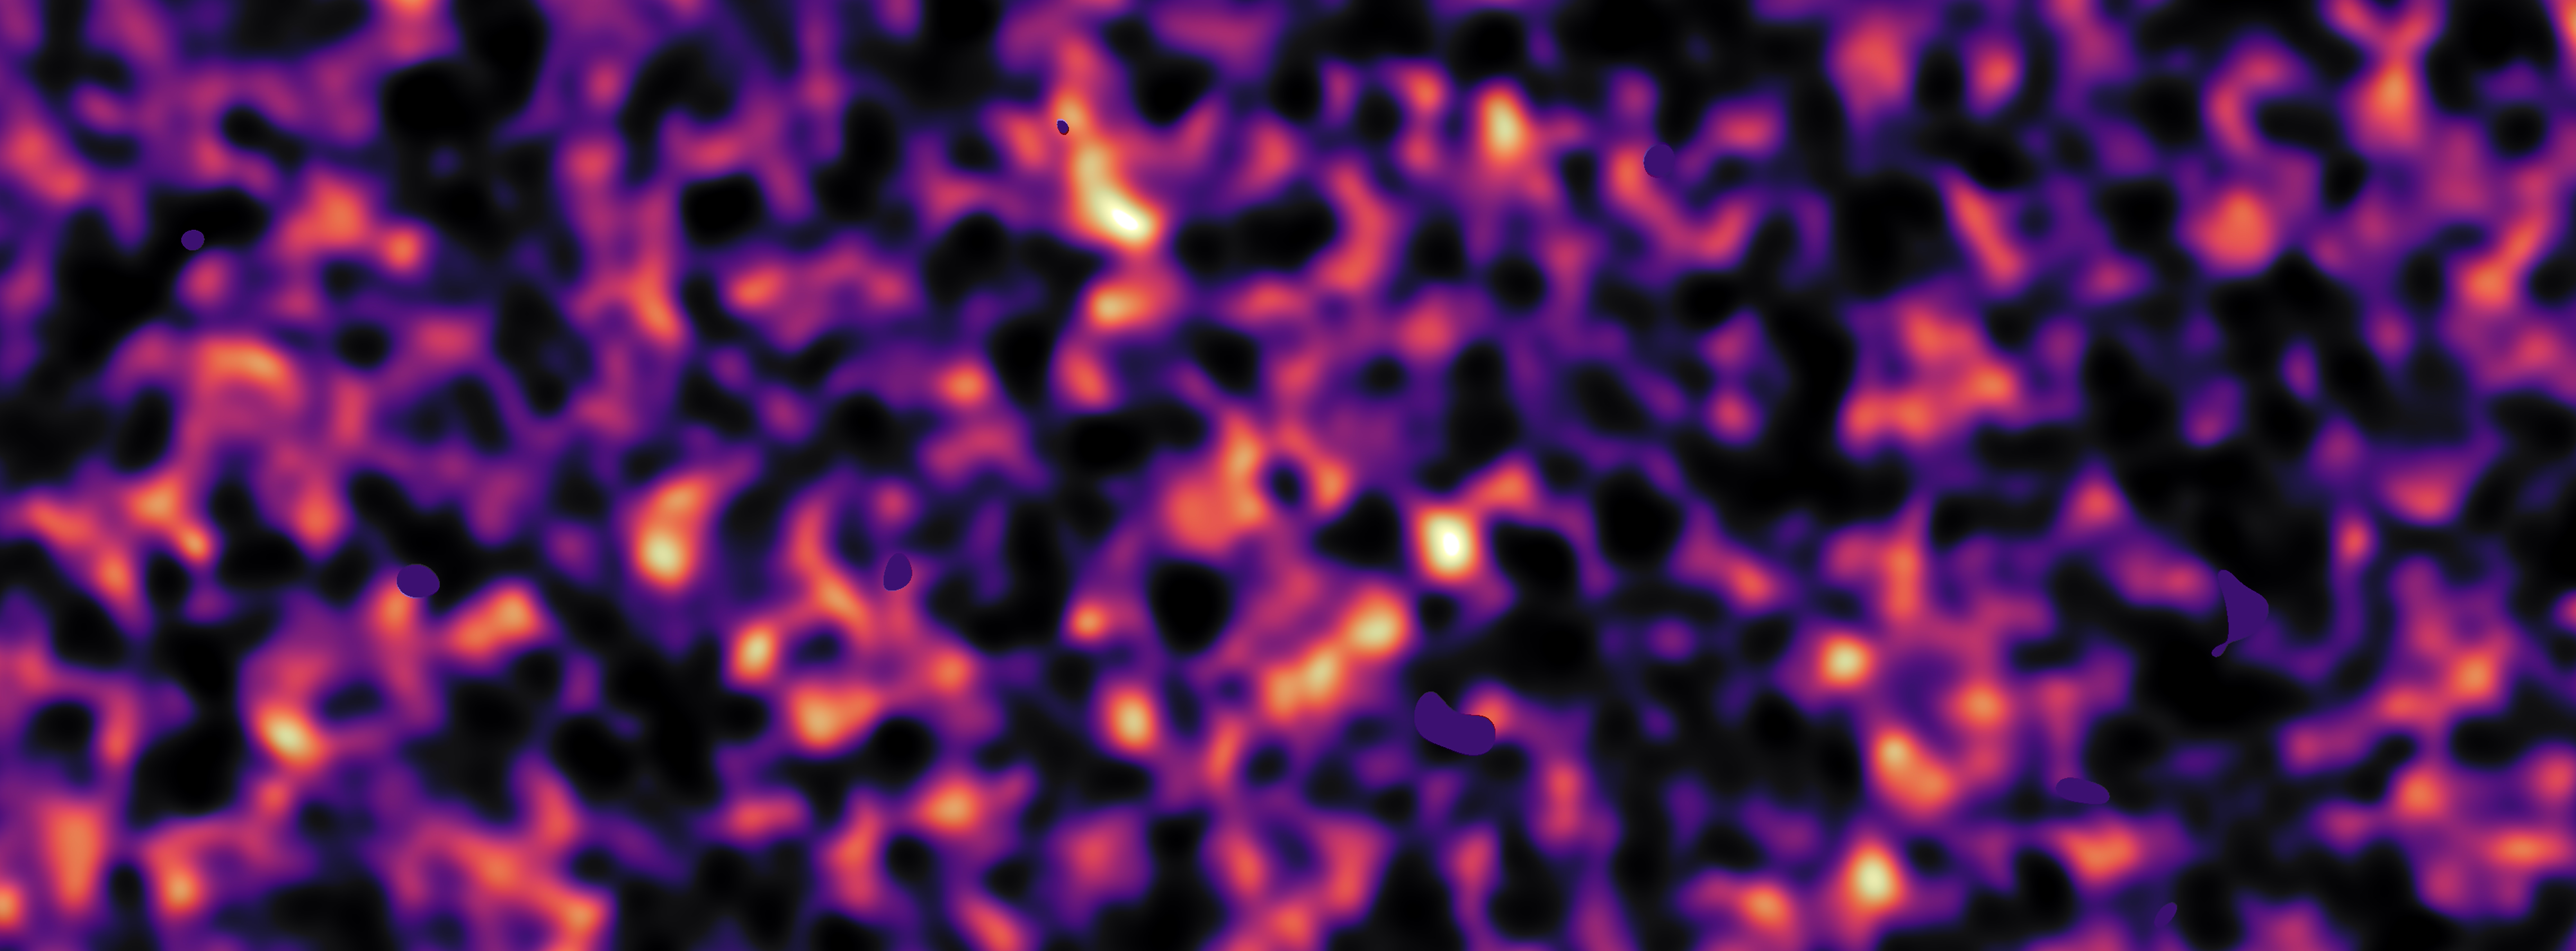
\includegraphics[width=1\linewidth]{Chap1/dark_matter_map.jpg}
    \caption{Dark matter map for a patch of sky based on gravitational lensing analysis of a Kilo-Degree Survey \cite{wikiDM}} 
    \label{fig:enter-label}
\end{figure}





\subsection{Observational Tests of the Dark Matter Scenario }  
Despite being invisible, dark matter has a substantial gravitational pull on visible matter and therefore numerous astrophysical observations have helped establish the existence of dark matter. A key early indication comes from observing the rotation curves of galaxies. According to Newtonian mechanics, stars and gas orbiting in a galaxy should slow down the farther they get from its center, where less mass is concentrated. But when we turn to observations of spiral galaxies, we find that stars at their outskirts are spinning, but they’re spinning far too quickly considering all the mass we can account for by the light produced from them. That implies the existence of more, unseen mass tugging on it gravitationally, a form of matter known as dark matter. The existence of this unseen mass, commonly known as the "dark halo," is required to account for both the observed flat rotation curves and the differences between predicted and actual stellar velocities within galaxies.

The Legacy of Gravitational Lensing is also a vital line of evidence for general relativity, the gravitational bending of light that Einstein’s 100-year-old theory predicts. When a beam of light from a very distant object such as a galaxy passes close to something big, like another galaxy cluster (or other matter of lesser mass), the path of that light beam gets bent and distorted, and you get warped looking images of background objects. The magnitude of this effect is directly related to the mass of the lensing body. Measurements of gravitational lensing around galaxy clusters provide evidence that the mass indicated by the lensing is much larger than that comprised only of visible matter contained in such clusters, implying that dark matter exists. One of the best known cases, the Bullet Cluster, has a separation between visible (X-ray) and dark matter (inferred from lensing), providing even more striking evidence for dark matter in galaxy clusters.\cite{clowe2006}

Evidence for dark matter The Big Bang left behind the Cosmic Microwave Background (CMB). These differences are those of temperature fluctuations of the CMB, which in turn reflect small density variations in the matter content and distribution of the early universe. These fluctuations are what enables cosmologists to infer the distribution of visible and invisible matter at that time. The results from the CMB, in particular the angular scale subtended by the first acoustic peak, provide extensive evidence for dark matter. Dark matter was essential for the gravitationally driven growth of cosmic structure that is encoded in the fluctuations in the CMB. By observing these fluctuations, researchers have measured the quantity of dark matter in the universe and verified its vital role in defining the cosmos.

Taken together, these three observational facts— galaxy rotation curves, gravitational lensing and Cosmic Microwave Background are a compelling suite of evidence for the reality of dark matter. Not only do they show that dark matter is critical for the creation of galaxies and galaxy clusters they also offer clues on what role it played in the early universe.

 

\subsection{Early Dark Matter Theories } 


It was around the early 20th century that scientists first began to realize that there were discrepancies between the motion of cosmic objects as they observed it and how much visible matter they could count. First evidence of what would eventually become known as dark matter comes from the research of the rotation curves of galaxies and member galaxy motions in clusters.

In 1933, the Swiss astronomer Fritz Zwicky observed one of the first pieces of evidence with dark matter. While observing the Coma galaxy cluster, Zwicky realized that galaxies in a cluster were moving at much higher velocities than could be explained by the matter we could see.\cite{zwicky1933} In terms of classical Newtonian mechanics, the gravitational attraction of the visible matter in the cluster should have decelerated the motions of galaxies and dispersed them until they could eventually escape from the cluster. But Zwicky’s measurements revealed that the total mass of the cluster didn’t suffice to explain what was keeping the galaxies tied up. He posited that there was a mysterious force of otherwise undetectable “missing mass” which was just sufficient to bind the galaxies. This “missing mass” would foreshadow the modern idea of dark matter. Zwicky even went so far as to call the substance “dunkle materie” or dark matter, although the idea went mostly unheralded at the time.\cite{zwicky1933}

The idea received a boost in the 1970s after astronomer Vera Rubin, building on Zwicky’s research, analyzed the rotation curves of galaxies.\cite{rubin1970} Rubin and her colleague Kent Ford discovered that stars on the outskirts of spiral galaxies were moving at unexpectedly high rates, given only the amount of visible matter in these galaxies. Also like Zwicky, Rubin determined that some type of dark or hidden mass must be exerting gravitational forces upon the stars in the arms, reinforcing her belief in the existence of dark matter. Her work was instrumental in placing dark matter at the center of modern cosmology.

When the notion of dark matter was first proposed, it originated from our inability to explain the motions of galaxies (as well as galaxy clusters) using gravity and regular baryonic matter alone, and scientists were free to imagine what kind of form this mysterious missing mass could take. It was speculated by some that it could be made up of ordinary, invisible or “dark” matter like faint stars or clouds of gas (so-called baryonic matter). But None of these is consonant with all the observed facts, notably the large structure of universe and detailed dynamics of galaxy clusters.

As dark matter was better understood, it turned out that it couldn’t just be regular old matter. This, in turn, eventually gave rise to the more sophisticated theories that exist today which postulate cosmological dark matter is primarily made of non-luminous, non-interacting particles. These particles (which interact via gravitational and, potentially, the weak force) give rise to more distinctive dark matter theories such as WIMPs and axions that will be discussed later in the section.

So, that's an overview of the early theories of dark matter which were developed mostly in response to astronomical data on galaxy and cluster motion. Zwicky and Rubin’s work helped establish the modern conception of dark matter as an essential part of the mass that makes up the universe, but what dark matter actually is would remain a mystery for decades.

 
 
\section{Problem Statement}
 The identification and characterization of dark matter are among the key open problems in astrophysics today. Novel approaches are required to overcome the absence of direct observational data. Machine learning can help us digest large complex datasets, allowing us to predict the properties and behaviors of dark matter. The goal of this proposal is to study the applicability of ML techniques on dark matter-related data and where possible discover new patterns/anomalies that would proof for such a distributed substance.

 

 
\subsection{Data Acquisition:}

In dark matter studies, the data acquisition is the essential part for collecting evidences to interpret this unknown and cold component of the universe. A spider web of cosmic proportions Because dark matter can’t be sensed directly, scientists employ a range of indirect means to gather information that might shed light on its existence, distribution and behavior. Such data are collected through astronomical observatories, space missions and with experiments aimed to detect the influences that dark matter has on visible materials and light.


Most of the data gathering in dark matter studies uses information from astronomy. Observations of galaxies, galaxy clusters and the like are needed to detect how dark matter’s gravitational clout impacts visible matter. Telescopes, on the ground and in space, provide data about how stars, gas and galaxies move. Notable examples include:

Rotation curves of galaxies: Measurements on galaxies rotation speeds that is evidence for dark matter halos. They are typically collected with optical and radio telescopes.

Gravitational Lensing: The deflection of light from faraway galaxies by the gravitational pull of dark matter in galaxy clusters. This is the data collected with optical and infrared telescopes including the Hubble Space Telescope and ESA's Gaia satellite.

Cosmic Microwave Background (CMB) satellite such as the Planck satellite have been measuring CMB-data, which is evidence for the structure of the early universe and how dark matter played a role in influencing its evolution. Temperature fluctuations in the CMB can be used to map matter density in the early universe.



 
\begin{figure}[H]
    \centering
    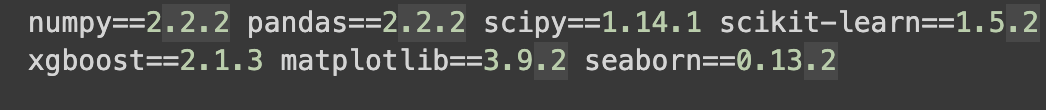
\includegraphics[scale=0.6]{Chap1/libraries.png}
    \caption{Necessary Libraries }
    \label{fig:my_label}
\end{figure}



\section{Motivation}
The origin of dark matter is one of the deepest questions in contemporary astrophysics and cosmology. Though postulated to exist, dark matter experiments have so far failed to detect this elusive substance. Observational evidence, such as galaxy rotation curves, gravitational lensing, and the cosmic microwave background indicates that it exists, but its precise nature is still unknown. This difficulty has pushed researchers to investigate new ways for analyzing data, among which ML are one of the most promising.

 



 
\section{Objectives} 
The goal of this effort is to use machine learning algorithms to predict and model various dark matter phenomena. Specific goals include:

\begin{itemize}
    \item To Estimate Dark Matter Distribution: Apply machine learning approaches to large-scale astronomical datasets and predict the spatial distribution of dark matter within galaxy clusters and in other cosmic structures.

    \item To Enhance Detection Sensitivity: Model machine learning algorithms which can enhance the sensitivity of the dark matter detection techniques like gravitational lensing, galaxy rotation curves and direct detection experiments.

    \item To Create Dark Matter Simulation: Develop computational tools that can predict the interactions of dark matter particles (e.g., WIMPs, axions) in different astrophysical environments so as to identify potential dark matter signatures.

    \item To Analyze Gravitational Effects: Analysis the influence of dark matter gravitational effect on visible stuff (e.g., their impact on galaxy motion, galaxy clusters and overall cosmic structures).

    \item To Develop and Enhance Data Analysis Techniques: Enhance techniques for analyzing large, intricate data sets from telescopes, experiments and simulations to identify dark matter signals more quickly and accurately.
\end{itemize}

\section{Scope of Work}
This web page will be useful as a strong tool to analyze the different profiles of dark matter by giving an easy platform for everyone in such a way that they can get knowledge about properties and behavior of the structures for dark matter. On-the-fly Shape Prediction Users work within a web-interface-based app to choose from several machine learning models such as Logistic Regression, SVM, Gradient Boosting and Random Forest in order to analyze and predict dark matter shapes given input data. It includes live visualizations, model performance comparison and prediction tools to let you evaluate your results using metrics like cross-validation accuracy.

 


 

\section{Outline}

In Chapter 2 a history of dark matter and current models followed by an introduction to the use of machine learning in astrophysics, with an emphasis on dark matter are discussed. It also sheds light on past research and its constraints.

Chapter 3 describes how we collected data, what machine learning models were used and the different types of pre-processing needed on the input signal, as well as how simulations are done around dark matter interactions. The machinery and technologies combined with the necessary tools used in the study.

Chapter 4 reports the machine learning results such as Dark Matter's Predictions. Contrasts the predictions of the model with existing observational data and performs sensitivity analysis to explore the robustness of results, interprets the cts, compares them with other observations and discusses their impact for dark matter searches. Discusses the implications of limitations met and recommendations for future research.

Chapter 5 summarizes the main results and contributions of the present work, pointing at machine learning as a promising tool for studying dark matter. Gives concluding remark on the future of dark matter research.

 

 
  










% \chapter{Literature Survey}
 
\chapter{Literature Review}
\label{chap:2}

\section{Overview} 

 This chapter introduces both dark matter and machine learning (ML) applications for astrophysics, and for dark matter studies in particular. The outline of this chapter is as follows: we first give the theoretical background of dark matter (Sect. 2), the role of machine learning in astrophysics (Sect. 3), and previous works that exploit ML for dark matter studies (Sect. 4). The present article provides a backdrop to the current study in the larger body of extant literature, recognizing opportunities and challenges while searching for gaps in knowledge.

\section{Introduction to Dark Matter}

This section gives a historical and theoretical introduction to the dark matter, as the search takes place in history of discovery and chronological series of developed models. Early theories, including those developed by Fritz Zwicky and Vera Rubin, are discussed, and then the present concept of dark matter as a fundamental feature of the universe is described. This part of the article also reviews as major candidates for dark matter, phenomenon like WIMPs (Weakly Interacting Massive Particles), axions and sterile neutrinos, noting the evidences that motivate their study from observation such as galactic rotation curves, gravitational lensing and CMB (Cosmic microwave background radiation).\cite{bertone2005,jungman1996}

\section{Machine Learning in Astrophysics} 

Machine learning in Astrophysics This section is primarily about how machine learning can be integrated into the field of astrophysical research. It presents the basics of ML and its rapidly growing importance for working with large, complex data sets which are typical in astronomy and cosmology. We compare different classes of machine learning algorithms (supervised, unsupervised and deep learning) as used for other astrophysical applications like star classification, galaxy morphology, cosmological simulations and so forth.\cite{wikiDM}

\section{Current Models for Dark Matter} 

Here we enter the chapter discussing some of those models that have been taken as benchmarks to describe dark matter and its properties. The standard cosmological model, the Lambda Cold Dark Matter (Lambda-CDM) model, is reviewed and its successes in explaining the large-scale structure of the universe are detailed.\cite{peebles1993,dodelson2003} The section also addresses alternative dark matter theories and models such as modified Newtonian dynamics, MOND that contest the Lambda-CDM model.\cite{famaey2012} The shortcomings of the existing models and the necessity for more sophisticated novel ones are also emphasized.

\section{Dark Matter Prediction via Machine Learning} 

In this section we describe some machine learning applied to dark matter analysis. Their applications include predicting the dark matter distributions in galaxy clusters, analyzing the rotation curves of galaxies and refining detection equipment for dark matter candidates such as WIMPs or axions. Past attempts of application of ML algorithms for the search of DM interactions in cosmic and laboratory experiments are subjected to a critical review.\cite{ackermann2015,fermilat2017} It also discusses how ML can be used to refine the dark matter models and enhance the sensitivity of current and future detection techniques.

\section{Quests for Dark Matter} 

In this section, we review all the major problems of dark matter search: the absence of direct detection, contractedness of dark matter theory and experimental methods. It also discusses the challenges of using machine learning in dark matter studies: complex data, overfitting and interpretability. The section will also discuss the ambiguities in DM candidates that hinder progress in the construction of model-dependent ML archetypes for particular kinds of DM.

\section{Summary and Knowledge Gaps}

A Summary of the Findings from Literature and Gaps on What Has Been Known Ultimately, it is important to summarize what are the specific findings and what we do not know about them. "The existence of measurements and accompanying limitations in our understanding thus far are the wellsprings for this dissertation, particularly those related to the use of machine learning methods in predicting dark matter distribution, boosting detection sensitivity, and simulating dark matter interaction." The section will stress the necessity of further research for ML to be able to contribute in advancing our knowledge about dark matter and the transformative possibilities arising from employing astrophysical observations and ML together.




%\chapter{Simulation Results and Discussion}
\chapter{Methodology}
\label{chap:3}

\section{Overview} 

Dark matter, an invisible material that comprises about 27 percent of the universe, has long been a focus of astrophysics research. It would be one of the important constituents of the universe, yet hitherto has escaped conventional detection. Dark matter is fundamental to explaining how galaxies form and the gravitational forces at work in the cosmos. The methods of study of the dark matter are based on complex analysis using supercomputers, data obtained from astronomical observations and advanced mathematical models. They are frequently based on Machine Learning (ML) algorithms aimed at helping to interpret complicated data and perform predictions of the behavior/properties of dark matter.



\section{Apparatus and Procedure for Computer Data Collection and Simulation}

For dark matter studies, data are usually obtained with sophisticated observatories and telescopes which combine multiple observations including galaxy clusters and gravitational lenses. Computer simulations are then employed to follow dark matter’s potential impact on these cosmic features. Such simulations provide a way to simulate under controlled conditions and powerfully test hypotheses about the nature of dark matter, in particular predicting how it interacts with visible matter and gravitational fields.

\section{Data Pre-processing}

Observational data obtained from different astronomical facilities may be noisy, not complete or in formats difficult to analyze. This data needs to be cleaned and processed before it is ready for analysis. Basics like cleaning noises, filling NAs, normalizing data are the most important step to avoid any distorted learning from ML models.
\section{Multivariate Analysis}
\begin{figure}[H]
    \centering
    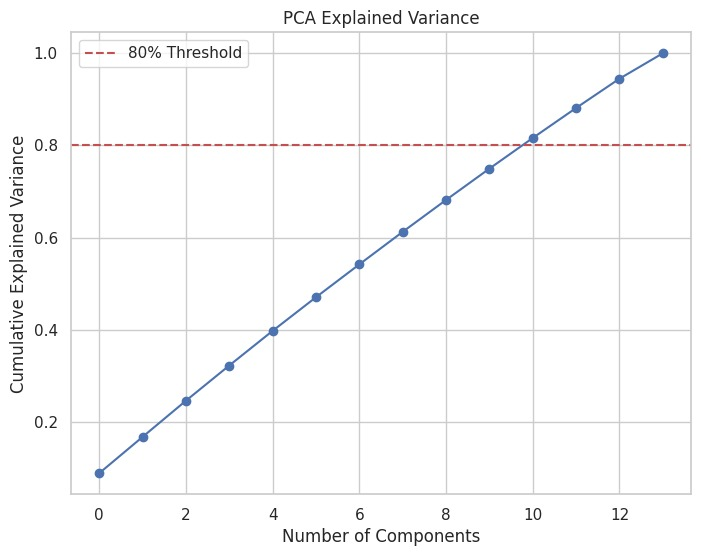
\includegraphics[width=1\linewidth]{Chap3/pca_explained_variance.jpeg}
    \caption{PCA Explained Variance}
    \label{fig:placeholder}
\end{figure}

This figure gives the Scree Plot, i.e. a cumulative variance plot of PCs from a PCA over a dataset.

\begin{itemize}
    \item The horizontal x-axis is the number of components, and the vertical y-axis is the cumulative explained variance.

    \item The figure reveals a continuous growth of the variance for higher and higher parts, that leads to a value close to 1.

    \item Above the plot a visible red line can be seen at 80\% which corresponds to what amount of variance (80\%) is represented by the respective principal components.
\end{itemize}
\begin{figure}[H]
    \centering
    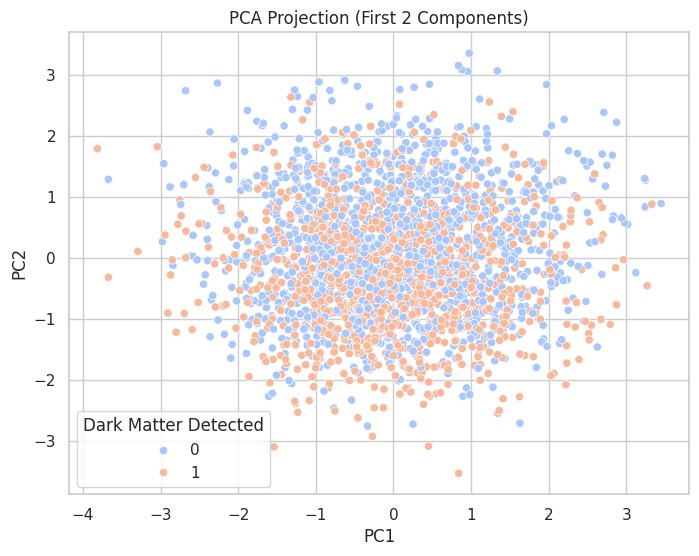
\includegraphics[width=1\linewidth]{Chap3/pca_projection.jpeg}
    \caption{First 2 component Projection}
    \label{fig:placeholder}
\end{figure}

This is a scatter plot that illustrates the data projected on to the first two principal components(PC1 and PC2) from PCA.

\begin{itemize}
    \item The x axis represents PC1 and the y axis denotes PC2.

    \item The data points are shaded whether or not dark matter is present, with blue representing "0" (no DM detection) and orange representing "1" (DM detection).

    \item This visualization allows checking how the first two components separate the two classes.
\end{itemize}
 
\section{Feature Selection and Engineering}

 

 \begin{figure}[H]
     \centering
     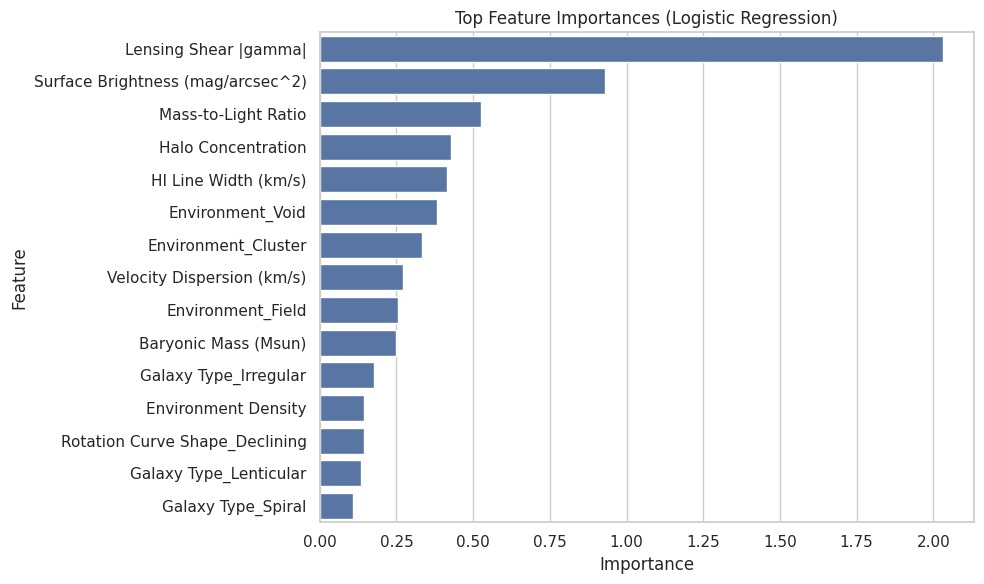
\includegraphics[width=1\linewidth]{image.png}
     \caption{Feature selection model}
     \label{fig:placeholder}
 \end{figure}
The chart you posted is the Top Feature Importances of a Logistic Regression model. It provides the importance of different features in predicting model output such as the length of bars suggest the corresponding significance.

\begin{itemize}
    \item The importance is highest for Lensing Shear [gamma]. This implies that gravitational lensing is the most important aspect of your model, meaning there is a strong correlation between lensing shear and the thing you are trying to predict (presumably dark matter or something like that)

    \item The Surface Brightness (mag/arcsec²) is next in priority. This means that the galaxies’ brightness per square arcsecond is an important factor in constraining the model’s prediction.

    \item Mass-to-Light Ratio and Halo Concentration are also big pieces of the puzzle, tells you that where the mass is as compared to light (how much dark matter there is relative to everything else) and how concentrated your galaxy’s halo matters.

    \item Other significant features are HI Line Width (km/s), Environment\_Void,Environment\_Cluster and Velocity Dispersion (km/s) that describe the environmental and dynamical properties of galaxies.

    \item Features such as Galaxy Type\_I rregular, Environment\_Density and Rotation Curve Shape\_Declining have some importance (ie contribute to the model) but they do it in a smaller way than the top features.

    \item Finally, Galaxy Type\_Lenticular and Galaxy Type\_Spiral have minor influence on the model performance,indicating that galaxy morphology may not be essential for this specific model.

\end{itemize}
 


\section{System Implementation}
\subsection{Performance Indicators}


Performance measures are critical to assess and compare the performance of machine learning model. They give the intuition about how well a model is doing on the problem you want it to solve. Performance measures comprise the accuracy, precision recall (sensitivity), F1 score, and model efficiency. And each of these metrics has a specific role to play in capturing some feature of the model behavior. These statistics are indispensable for both evaluating and refining the model to achieve optimal performance in a particular task.


\subsection{Analysis of the Confusion Matrix} 
The confusion matrix is a widely used technique to evaluate the classification models. It does gives a good in-depth breakdown of the true positives, true negates, false positives, and falls negatives. We can use the confusion matrix to compute a lot of performance metrics like accuracy, precision, recall and F1 score. The confusion matrix is a visual representation of how well the model is doing for classifying data to different classes, it makes it easy to identify where the model might be going wrong. This matrix is fundamental to interpret the strengths and weaknesses of the model on different category predictions.

 


\subsection{Accuracy}

Accuracy is the easiest and most straightforward performance measure. The ratio of correct predictions (True Positive + True Negative) to the total number of predictions made. On the other hand, accuracy provides a fast—but incomplete—picture of how a model is performing and can be misleading if the dataset is unbalanced. For example, in a very imbalanced dataset the model which always predicts the majority class can have high accuracy yet still suck at finding the minority class. Thus, accuracy should not be viewed in isolation but studied along with other metrics to have an integrated view of a model's performance.


\subsection{Precision}
Precision, just as a reminder that it’s sometimes called positive predictive value as well, is the rate at which our classifier generates true positives. It addresses the question: of all positive predictions by the model, how many were positive? Accuracy is crucial when false positives are cost-prohibitive or unjustifiable. If, say, a medical diagnosis model misclassifies healthy people as sick, it could prompt unnecessary tests or treatments. High precision indicates high trust in positive predictions.
\begin{table}[H]
\centering
\begin{tabular}{|l|c|c|}
\hline
\textbf{Model} & \textbf{Precision (0)} & \textbf{Precision (1)} \\
\hline
Decision Tree       & 0.76 & 0.71 \\\hline
Gradient Boosting   & 0.81 & 0.79 \\\hline
KNN                 & 0.73 & 0.72 \\\hline
Logistic Regression & 0.82 & 0.81 \\\hline
Naive Bayes         & 0.78 & 0.82 \\\hline
Random Forest       & 0.79 & 0.77 \\\hline
SVM                 & 0.79 & 0.77 \\\hline
XGBoost             & 0.79 & 0.76 \\
\hline
\end{tabular}
\caption{Precision for each model}
\end{table}





\subsection{Recall or Sensitivity}

Recall, or sensitivity, indicates the percentage of true positive instances that were accurately predicted by the model. e. true positives) the model was able to identify? Recall is particularly significant in the presence of severe costs associated with missing positive cases. For instance, in a fraud detection system not detecting fraudulent transactions (false negatives) might result in large losses. High recall means the model is catching as many of the true positive results as possible.
\begin{table}[H]
\centering
\begin{tabular}{|l|c|c|}
\hline
\textbf{Model} & \textbf{Recall (0)} & \textbf{Recall (1)} \\
\hline
Decision Tree       & 0.68 & 0.79 \\\hline
Gradient Boosting   & 0.78 & 0.82 \\\hline
KNN                 & 0.72 & 0.74 \\\hline
Logistic Regression & 0.80 & 0.82 \\\hline
Naive Bayes         & 0.83 & 0.77 \\\hline
Random Forest       & 0.76 & 0.80 \\\hline
SVM                 & 0.76 & 0.79 \\\hline
XGBoost             & 0.75 & 0.80 \\
\hline
\end{tabular}
\caption{Recall for each model}
\end{table}



\subsection{\textbf{F1 Score}}
The F1-score is the harmonic mean of precision and recall. It is a compromise between precision and recall that weights the two equally. F1 score is especially helpful when you have an uneven class distribution and moreover false positive and false negatives are of significant cost. Unlike accuracy which can be affected by a class imbalance, F1 score takes into account both the ability to identify positive cases (recall) and whether the predictions are correct or not (precision). A high F1 score means a model with good precision and recall.
 \begin{table}[H]
\centering
\begin{tabular}{|l|c|c|}
\hline
\textbf{Model} & \textbf{F1-Score (0)} & \textbf{F1-Score (1)} \\
\hline
Decision Tree       & 0.72 & 0.75 \\\hline
Gradient Boosting   & 0.79 & 0.80 \\\hline
KNN                 & 0.73 & 0.73 \\\hline
Logistic Regression & 0.81 & 0.82 \\\hline
Naive Bayes         & 0.80 & 0.79 \\\hline
Random Forest       & 0.77 & 0.79 \\\hline
SVM                 & 0.77 & 0.78 \\\hline
XGBoost             & 0.77 & 0.78 \\
\hline
\end{tabular}
\caption{F1-Score for each model}
\end{table}








%Chapter{Performance Analysis}
\chapter{Observations}
 %This section  .... table \ref{table:2} \cite{r2}
\section{Insights from Computational Analysis} 

From the computation results, it is clear that Logistic Regression performs better than other models, and gains the top CV accuracy of 90.11\%. This indicates that Logistic Regression gives the highest generalization performance over all of the models. SVM is a close second with CV accuracy of 88.52\%, showing that it is good at learning digest intricate information in the data. Gradient Boost, Random Forest, XGBoost and Naive Bayes  classifiers also yield comparable performance (87\%-80.0\% CV accuracies). These models work well, though they don’t take the top two spots. Here by comparing the CV accuracies, we notice that SVM does fairly close at 88.52\% and KNN and Decision Tree have significantly lower CV accuracies of 80.5\% and 72.57\% respectively meaning that they do worse in generalizing on unseen data than the other methods.




\section{Limitations} 

Models have different capabilities but there are a number of limitations. First, the analysis was made using cross-validation accuracy and not the whole model performance. Class imbalance, overfitting or data-specif characteristics in the domain can have an impact on their performance when employed in deployment. Also, the method does not consider hyperparameter tuning for each model. These can potentially improve the performance of the methods. Finally, the model complexity and explainability of some models such as Gradient Boosting and XGBoost can make them less useful in practice for certain problem settings than simpler models like Logistic Regression or Naive Bayes.


\section{Results}



The results of our experiments (cross-validation accuracies) suggest that Logistic Regression and SVM are the two top models for this task. These are both reasonably simple yet powerful models, that were shown to achieve high accuracy with low computational cost. We find that Naive Bayes, Gradient Boosting and Random Forest give good results but not better than Logistic Regression and SVM in our context. The KNN and Decision Tree methods are outperformed by the latter, and it may indicate that more complex techniques suit to the specific nature of this problem better, probably because they capture intricate patterns/interplays present in the data.

\begin{table}[ht]
\centering
\begin{tabular}{|l|c|}
\hline
\textbf{Model}            & \textbf{CV Accuracy} \\ \hline
Logistic Regression        & 0.90              \\ \hline
SVM         & 0.86              \\ \hline
Gradient Boosting                & 0.88              \\ \hline
Random Forest                         & 0.88              \\ \hline
XGBoost             & 0.88              \\ \hline
Naive Bayes                    & 0.87              \\ \hline
KNN                         & 0.80              \\ \hline
Decision Tree              & 0.73              \\ \hline
\end{tabular}
\caption{Cross-Validation Accuracy of Various Models}
\label{tab:cv_accuracy}
\end{table}

 
\begin{figure}
    \centering
    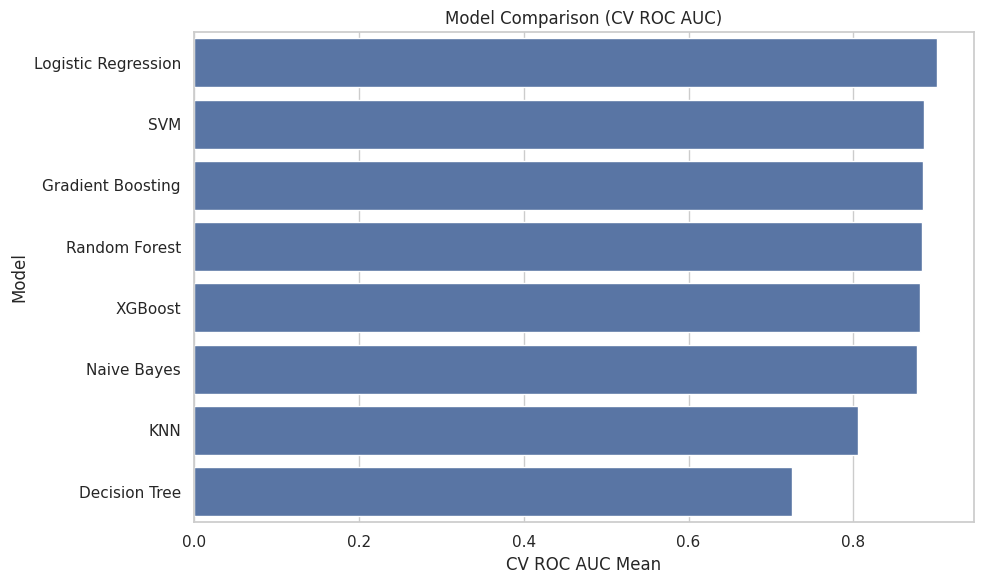
\includegraphics[width=0.75\linewidth]{Chap4/model-comparision.png}
    \caption{Compare model}
    \label{fig:placeholder}
\end{figure}

\section{Web Application}
\begin{figure}
    \centering
    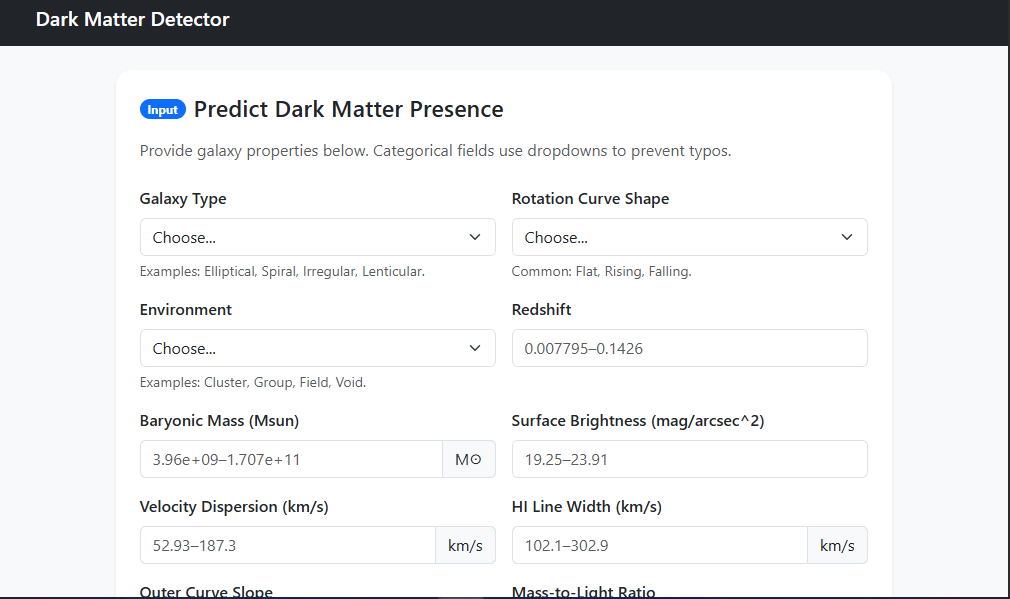
\includegraphics[width=0.5\linewidth]{Chap4/web-application.png}
    \caption{Web application of dark matter detector}
    \label{fig:placeholder}
\end{figure}
The Dark Matter Detector site is a web based, freely available tool that uses a very user-friendly and intuitive user interface to calculate the probability dark matter is detected given arbitrary date for R V, Reff, $\Sigma$g ±. The features to be chosen by the user for classification are basic properties of a galaxy such as its type (e.g., Elliptical, Spiral, Irregular or Lenticular) and nature of environment it reside in –cluster, group, field or void. And, users can provide their baryonic mass in solar masses, the velocity dispersion in km/s and the outer curve slope, which is a good representation of how the rotation curve of your galaxy behaves at its outskirts.

Other important parameters are the rotation curve type (flat, rising, falling, etc.) and whether or not we need to plot a gap (it can highlight with clip marks if you select yes). The redshift is another important parameter that shows the distance and motion of galaxy with respect to Earth. The surface brightness S in units of magnitudes per square arc-second and the HI line width provide an estimate of the galaxy luminosity and also on velocity distribution of hydrogen gas inside a galaxy. Finally, the user must specify the mass-to-light ratio, an important parameter in determining how much dark matter there is on the basis of its visible mass and the gravitational impact of the galaxy.

By imputing these galaxy properties, the website hopes to make a prediction for the probability of dark matter presence and contribute to human understanding of how a galaxy’s visible properties relate to the invisible substance that determines its evolution. This is an essential tool to push forward the field of dark matter astrophysics.

 


%\chapter{Conclusion and Future Work}
\chapter{Conclusion and Future Work}

\section{Conclusion}
Dark matter is the dominant mystery of today’s astrophysics and cosmology. It is invisible as it cannot be detected by indirect means, and we instead infer its existence from the effect of gravity on visible matter like galaxies and galaxy clusters. Through the observation of cosmic structures (such as galaxy-wide rotation curves, gravitational lensing, and the first acoustic peak in the CMB), scientists' estimates for dark matter changed to approximately 27\% of mass-energy content. But it is not clear what exactly, with weakly interacting massive particles (WIMPs), axions and sterile neutrinos, some of the most likely candidates.

Much progress has been made and new technologies have been developed over the years, but dark matter, mapped in detail or detected directly, remains elusive, resisting all particle physics and cosmological theories to date. Understanding dark matter is important not just for understanding how the universe is built, but also for revealing the very substance of physics at its deepest scale.

\section{Limitation}

\begin{itemize}
    \item \textbf{Quality and Availability of Data:}Reliance on good quality data being available, many cosmic surveys can limit accuracy.

    \item \textbf{Computation Constraints:} Precise models require large amount of computation resources, thus cannot be scalable.

    \item \textbf{Dependence on the Model:} Not all nuances of sequences might be optimally captured by models, in particular with noisy or scarce data.

    \item \textbf{Generalisation: }The results might be dataset dependent and not applicable for any analysis of dark matter.
\end{itemize}


 
\section{Potential Improvements}
Enhanced Detection Techniques: Increasing the sensitivity and resolution of detectors for detecting dark matter will be critical for observing a rare interaction between dark matter particles and ordinary matter. Advances in cryogenic detectors, liquid xenon detectors and high energy particle accelerators may offer the next leap in direct detection.

\begin{itemize}
    \item Better Data From Space: Observatories in space, like the James Webb Space Telescope and the upcoming LISA mission, might provide more information about how dark matter is distributed in the cosmos and how it interacts with ordinary matter. Sharper observations of galaxy clusters and gravitational lensing will better map dark matter in the future.

    \item Interdisciplinary Methods Jointly studying particle physics, astronomy, and cosmology will help achieve more comprehensive insights into dark matter. Cooperation between theoretical physicists and observational astronomers will be crucial for testing the current hypotheses and even to provide new models of dark matter.

    \item Alternative Theories and Models Continuing to explore alternative theories of dark matter can serve two purposes toward the goal of gaining more insight into its nature: one is to constrain or rule out such models, and the other is an opportunity for discovering new physics.
    \item 
\end{itemize}
In summary, although dark matter remains a persistent enigma, there are reasons for optimism as improved detection technology, theoretical modeling and observations continue to improve the prospects for major discoveries in the coming years. It can be expected that a determination of the nature of dark matter will have far-reaching consequences for both cosmology and particle physics, altering our conception of the universe.

 
% \label{chap:conclusion}
% \chapter{Conclusion and Future Work}

\section{Conclusion}
Dark matter is the dominant mystery of today’s astrophysics and cosmology. It is invisible as it cannot be detected by indirect means, and we instead infer its existence from the effect of gravity on visible matter like galaxies and galaxy clusters. Through the observation of cosmic structures (such as galaxy-wide rotation curves, gravitational lensing, and the first acoustic peak in the CMB), scientists' estimates for dark matter changed to approximately 27\% of mass-energy content. But it is not clear what exactly, with weakly interacting massive particles (WIMPs), axions and sterile neutrinos, some of the most likely candidates.

Much progress has been made and new technologies have been developed over the years, but dark matter, mapped in detail or detected directly, remains elusive, resisting all particle physics and cosmological theories to date. Understanding dark matter is important not just for understanding how the universe is built, but also for revealing the very substance of physics at its deepest scale.

\section{Limitation}

\begin{itemize}
    \item \textbf{Quality and Availability of Data:}Reliance on good quality data being available, many cosmic surveys can limit accuracy.

    \item \textbf{Computation Constraints:} Precise models require large amount of computation resources, thus cannot be scalable.

    \item \textbf{Dependence on the Model:} Not all nuances of sequences might be optimally captured by models, in particular with noisy or scarce data.

    \item \textbf{Generalisation: }The results might be dataset dependent and not applicable for any analysis of dark matter.
\end{itemize}


 
\section{Potential Improvements}
Enhanced Detection Techniques: Increasing the sensitivity and resolution of detectors for detecting dark matter will be critical for observing a rare interaction between dark matter particles and ordinary matter. Advances in cryogenic detectors, liquid xenon detectors and high energy particle accelerators may offer the next leap in direct detection.

\begin{itemize}
    \item Better Data From Space: Observatories in space, like the James Webb Space Telescope and the upcoming LISA mission, might provide more information about how dark matter is distributed in the cosmos and how it interacts with ordinary matter. Sharper observations of galaxy clusters and gravitational lensing will better map dark matter in the future.

    \item Interdisciplinary Methods Jointly studying particle physics, astronomy, and cosmology will help achieve more comprehensive insights into dark matter. Cooperation between theoretical physicists and observational astronomers will be crucial for testing the current hypotheses and even to provide new models of dark matter.

    \item Alternative Theories and Models Continuing to explore alternative theories of dark matter can serve two purposes toward the goal of gaining more insight into its nature: one is to constrain or rule out such models, and the other is an opportunity for discovering new physics.
    \item 
\end{itemize}
In summary, although dark matter remains a persistent enigma, there are reasons for optimism as improved detection technology, theoretical modeling and observations continue to improve the prospects for major discoveries in the coming years. It can be expected that a determination of the nature of dark matter will have far-reaching consequences for both cosmology and particle physics, altering our conception of the universe.

 

%\startbibliography
 %\begin{singlespace} % Bibliography must be single spaced
%\bibliography{References}   % Use the BibTeX file ``References.bib''.


%\end{singlespace}
%%\setlinespacing{1.44}
% \bibliographystyle{ieeetr}
\bibliographystyle{unsrt}
\bibliography{darkmatter}
\end{document}